\documentclass[11pt,a4paper]{article}

\usepackage[T1]{fontenc}
\usepackage[utf8]{inputenc}
\usepackage{lmodern}
\usepackage[margin=2.5cm]{geometry}
\usepackage{amsmath,amssymb}
\usepackage{booktabs,tabularx,multirow}
\usepackage{graphicx}
\usepackage[font=small,labelfont=bf]{caption}
\usepackage[round,authoryear]{natbib}
\usepackage{microtype}
\usepackage{xcolor}
\usepackage[hidelinks]{hyperref}
\usepackage{url}
\defcitealias{koeri_ko}{KOERI, 1971}
\defcitealias{afad_catalog}{AFAD, 2026}

\newcommand{\fc}{f_c}
\newcommand{\code}[1]{\texttt{\detokenize{#1}}}
\newcolumntype{L}{>{\raggedright\arraybackslash}X}

\title{Amplitude-Independent Waveform Descriptors\\ of Earthquake Size:
A Leakage-Controlled\\ Gradient-Boosting Study on Turkish Broadband Data}
\author{[Student name]\thanks{[Department, University]. Supervisor: [Advisor name].}}
\date{Preliminary report --- October 2026}

\begin{document}
\maketitle

\begin{abstract}
\noindent
Most data-driven magnitude estimators exploit recorded amplitude, which is the
quantity magnitude scales are defined from. This study asks how much
information about earthquake size remains in a seismogram once absolute
amplitude, and every quantity that acts as an amplitude proxy, is removed, and
which physical measurement carries it. From 78\,732 three-component
broadband records of 11\,758 earthquakes ($M \geq 2.0$) recorded by the KOERI
network in 2025--2026, 131 descriptors were extracted, each constructed to be
invariant to a rescaling of the record and none referenced to the pre-event
noise. A within-event audit removed 79 descriptors whose values tracked
station signal-to-noise ratio. Gradient-boosted regression trees were trained
on a magnitude-balanced, spatially de-clustered subset of 3\,697 events and
evaluated on folds that share neither events nor stations with the training
data. The amplitude-independent model reached an event-level mean absolute
error of $0.343 \pm 0.017$ magnitude units, compared with $0.392 \pm 0.016$ for
source--station geometry alone and $0.238 \pm 0.022$ for a reference model given
peak amplitude, i.e.\ it recovered about one third of the gap between the two.
Permutation tests identify the network-median, attenuation-corrected
corner frequency of P and S waves as the dominant descriptor, ahead of
source--station distance. Its scaling with magnitude, however, is
much shallower than self-similar source theory predicts, indicating a
band-limited apparent corner frequency; correspondingly, all models
underestimate events above $M\,3.5$. These results are preliminary.
\end{abstract}

\section{Introduction}

Earthquake magnitude scales are defined from amplitudes: local magnitude
$M_L$ from the peak of a simulated Wood--Anderson record, moment magnitude
$M_w$ from the low-frequency level of the displacement spectrum
\citep{hanks1979}. Machine-learning estimators trained on raw waveforms
inherit this definition and learn primarily from amplitude, either
explicitly or through normalisation choices that preserve it
\citep{mousavi2020,mousavi2023}. Such estimators are accurate, but they
answer a narrow question and are exposed to the weaknesses of amplitude:
instrument gain and site amplification errors, clipping near large events,
and saturation of early, short windows.

Source physics predicts that earthquake size also controls the
\emph{shape} of a seismogram. Larger ruptures last longer and radiate
relatively more low-frequency energy, which lowers the corner frequency of
the source spectrum \citep{brune1970,boatwright1980,abercrombie1995}.
Period parameters used in earthquake early warning exploit the same
principle from the first seconds of the P wave \citep{allen2003,kanamori2005,wu2005}.
These shape descriptors are, however, entangled with propagation (attenuation,
distance) and with the noise floor of weak records, so a data-driven model
can easily appear to learn ``shape'' while in fact recovering amplitude.

This study therefore asks two questions: \textbf{(i)} how much information
about magnitude is retained by waveform descriptors that are provably
insensitive to amplitude and empirically insensitive to signal-to-noise
ratio, and \textbf{(ii)} which physical descriptor carries that information.
The contributions are:
\begin{itemize}
\item a feature set of 131 descriptors, each invariant to a rescaling of the
  record by construction and verified by an automated test, including
  physics-based source, period and duration parameters;
\item a within-event leakage audit that separates noise-floor sensitivity from
  genuine source variation, and is applied by default;
\item a magnitude-balanced, spatially de-clustered event selection and a
  doubly disjoint (event and station) validation design with explicit
  geometric and amplitude reference models;
\item a ranking of descriptors by grouped permutation importance, which
  identifies the corner frequency, corrected for attenuation, as the main
  carrier of size information.
\end{itemize}

\section{Background and preliminary literature review}
\label{sec:lit}

\emph{Note.} At the time of writing the author had no institutional access
to full texts. The review below relies on abstracts, publisher metadata and
established textbook knowledge; all bibliographic data were verified against
Crossref or publisher records (see the declaration in
Section~\ref{sec:ai}). Statements should be checked against the original
papers before formal submission.

\subsection{Magnitude scales and source scaling}
Moment magnitude is tied to the static seismic moment \citep{hanks1979}.
Local magnitude, by contrast, is a dynamic, high-frequency measure;
\citet{deichmann2006} showed theoretically that the two scales diverge for
small earthquakes, whose corner frequencies lie above the passband of the
Wood--Anderson response. Since the AFAD catalogue reports $M_L$ for most
events in this study and $M_w$ for larger ones, the target variable is a mixture
of the two scales. In the $\omega^{2}$ source model \citep{brune1970} the
displacement spectrum is flat below the corner frequency $\fc$ and decays as
$f^{-2}$ above it. Under constant stress drop (self-similarity),
$M_0 \propto \fc^{-3}$, i.e.\ $\log_{10}\fc$ decreases by $0.5$ per unit $M_w$.
Self-similarity of small earthquakes has been supported by borehole
recordings down to very small magnitudes \citep{abercrombie1995} and by
stacked P and S spectra of southern California earthquakes
\citep{prieto2004}, although the question remains debated.

\subsection{Spectral source parameters and attenuation}
Observed spectra combine source, path and site. High-frequency decay near the
receiver is commonly modelled by the parameter $\kappa$ \citep{anderson1984};
for the Marmara region, \citet{sertcelik2022} reported a dependence of
$\kappa$ on magnitude, which illustrates how strongly source and attenuation
effects are coupled. Parametric source fits include the Brune model and the
generalised fall-off model of \citet{boatwright1980}. A non-parametric
alternative replaces the fitted corner by the ratio of spectral integrals of
velocity and displacement \citep{andrews1986,snoke1987}, which is more stable
for band-limited data. Frequency-dependent attenuation in Anatolia is strong:
$Q_S \approx 40 f^{1.03}$ was reported for the Sea of Marmara
\citep{horasan2004}, and coda $Q_c \approx 57.5 f^{0.82}$ for the East Anatolian
Fault Zone \citep{sertcelik2012}. At magnitudes 2--3 the expected corner
frequencies (of order 10\,Hz or more) fall in the band where such attenuation
removes most energy over typical regional distances.

\subsection{Period and duration parameters from early warning}
Earthquake early warning estimates size from the first seconds of P. The
recursive predominant period $\tau_p^{\max}$ \citep{allen2003} and the
effective period $\tau_c$ \citep{kanamori2005,wu2005} are ratios of signal
moments and therefore independent of amplitude; \citet{olson2005} argued from
such observations that final size is partly determined early in the rupture.
\citet{colombelli2015} showed that the logarithm of peak P displacement as a
function of time (LPDT) grows and then levels off, and related the corner
time of this curve to the rupture half-duration. Significant duration, the
interval over which normalised cumulative energy grows from 5 to 95\,\%
\citep{trifunac1975}, is likewise amplitude-free, and modern duration models
parameterise its magnitude dependence through source duration
\citep{afshari2016}.

\subsection{Machine-learning magnitude estimation}
Deep networks trained on single-station waveforms estimate local magnitude
with small error \citep{mousavi2020,lomax2019}, and multi-station transformer
models have been developed for early warning \citep{munchmeyer2021}; see
\citet{mousavi2023} for a review. These models are designed to use amplitude
and are not intended to separate it from other information. Gradient-boosted
decision trees \citep{ke2017} on engineered features offer a transparent
alternative, for which exact tree-based Shapley values \citep{lundberg2020} and
permutation importance \citep{breiman2001} are available; for correlated
features, conditional or grouped schemes are preferable
\citep{strobl2008}.

\subsection{Leakage and structured validation}
Leakage, information about the target entering through an unintended route,
inflates apparent skill \citep{kaufman2011}, and models readily exploit such
shortcuts \citep{geirhos2020}. For data with spatial and hierarchical
structure, random cross-validation is optimistic and blocked designs are
recommended \citep{roberts2017}. In this problem, amplitude can leak through
signal-to-noise-dependent shapes, station selection and catalogue metadata,
and site response can leak across folds that share stations.

\subsection{Gap addressed}
To the author's knowledge, the literature reviewed here does not quantify how
much magnitude information remains when amplitude and its proxies are removed
by construction and audited empirically, nor ranks physically interpretable
descriptors under a validation design that excludes shared events and shared
stations. A systematic literature search with full-text access is required to
confirm this assessment.

\section{Data}
\label{sec:data}

Hypocentres and magnitudes were taken from the AFAD earthquake catalogue
\citepalias{afad_catalog}. Waveforms are continuous 100\,Hz three-component
broadband (HH) recordings of the KOERI network \citepalias{koeri_ko}, cut from 60\,s
before to 120\,s after each catalogue origin time, together with station
coordinates. Windows were available for 12\,617 catalogue events with
$M \geq 2.0$ between May 2025 and August 2026. Magnitudes are reported to
0.1 units (12\,257 $M_L$, 360 $M_w$) and origin times to whole seconds.
The magnitude distribution is strongly skewed: the median is 2.3 and about
70\,\% of events lie between 2 and 3 (Figure~\ref{fig:selection}).

\section{Methodology}
\label{sec:method}

\subsection{Pre-processing, travel times and P picking}
For each event and station the first instrument with three components was
selected (HH in all retained records). Segments were merged, and any gap inside the
required time span rejected the record. Theoretical first P and S arrivals
were interpolated from a table of the iasp91 model \citep{kennett1991} computed
with TauP \citep{crotwell1999} as implemented in ObsPy \citep{beyreuther2010}.
The required span was demeaned, linearly detrended, tapered (5\,\% cosine)
and filtered with causal fourth-order Butterworth filters: a 1--40\,Hz band-pass
for time-domain descriptors and picking, and a 0.5\,Hz high-pass for spectra
and period parameters. Causal filters were used so that no energy is
displaced ahead of the onset. Instrument response was not removed; the
broadband response is flat over the band used, and constant gain factors
cancel in all descriptors (Section~\ref{sec:invariance}).

The P onset was refined with the Akaike-information-criterion picker of
\citet{maeda1985} on the band-passed vertical component, searching from 1.5\,s
before to 3\,s after the theoretical arrival (and at least 0.3\,s before the
theoretical S). The asymmetric window accounts for catalogue origin times
being given to whole seconds: in a 200-event trial the median pick
lay 0.75\,s after the theoretical time, approximately independent of distance,
while the picker was unbiased on synthetic records. The S time was set to the
picked P time plus the theoretical S--P interval.

\subsection{Windows and quality control}
Fixed windows relative to the picks were used throughout (Table~\ref{tab:windows}),
so that spectral resolution and statistics are comparable between records.
A record was rejected if it was clipped (absolute count $\geq 8\times10^{6}$, or at
least five samples at the peak value), or if the root-mean-square
signal-to-noise ratio (SNR) in the P or S window, relative to a noise window
ending 1\,s before P, was below 3. SNR was used only for this gate and for the
audit below, never as a model input.

\begin{table}[ht]
\centering\small
\caption{Analysis windows ($t_P$: picked P time; $t_S$: derived S time).}
\label{tab:windows}
\begin{tabular}{lll}
\toprule
Window & Span & Components \\
\midrule
Noise (QC only) & $[t_P-6,\ t_P-1)$\,s & all \\
P & $[t_P-0.05,\ t_P+1.95)$\,s (200 samples) & Z \\
S & $[t_S-0.2,\ t_S+4.8)$\,s (500 samples) & N, E \\
Polarisation & first 1\,s of the P and S windows & Z, N, E \\
Envelope & $[t_P-1,\ t_S+10)$\,s & horizontal \\
LPDT & $[t_P,\ t_P+\min(3,\ t_S-t_P-0.2))$\,s & Z \\
\bottomrule
\end{tabular}
\end{table}

\subsection{Amplitude invariance and the leakage audit}
\label{sec:invariance}
Every descriptor is computed after normalising each window by its own
peak, and is either a ratio of quantities of equal degree in amplitude, a time
or frequency read from a normalised curve, an ordinal statistic, or a fitted
shape whose level parameter is discarded. Consequently, multiplying a record
by any constant $c \neq 0$ leaves every descriptor unchanged. This property was
verified by an automated test on synthetic three-component records for
$c \in \{10,\ 0.01,\ -3\}$; the case $c=-3$ led to the use of the absolute value of
skewness, whose sign reflects polarity rather than size.

Invariance does not exclude indirect leakage: a fixed-length window on a weak
record contains relatively more noise, so spectral and envelope shapes can
encode SNR, and thereby amplitude. Partial correlation with SNR at fixed
catalogue magnitude is an unsuitable test, because catalogue magnitudes are
uncertain and a genuinely larger event has both higher SNR and a lower corner
frequency. The audit therefore operates \emph{within events}, where the source
is identical. Ranks of a descriptor $x$, of $\log_{10}$SNR and of
$\log_{10}$ hypocentral distance $r$ are demeaned per event; $x$ and SNR are then
residualised on $r$, and the leakage score is
\begin{equation}
  \lambda(x) = \max_{w\in\{P,S\}} \left| \operatorname{corr}\!\left(\tilde x,\ \widetilde{\log \mathrm{SNR}_w}\right) \right| ,
\end{equation}
the larger absolute within-event partial rank correlation with the P- and
S-window SNR. Descriptors with $\lambda > 0.15$, or with an undefined score, are
excluded by default; the audit is recomputed on each training set. The
threshold removed 79 of 131 descriptors, among them all permutation-, sample-
and SVD-entropy and fractal-dimension measures, all significant-duration
measures, $\tau_c$ and $\tau_p^{\max}$, the vertical-component envelope
descriptors, and the fitted Brune and Boatwright corner frequencies, fall-off
exponents and $\kappa$ values. The retained descriptors have a median
$\lambda$ of 0.07 (maximum 0.147). Only results obtained with this filter are
reported.

\subsection{Descriptors}
Table~\ref{tab:features} summarises the families; all 131 are defined in the
project documentation and the 52 retained ones are listed in
Appendix~\ref{app:features}. The key definitions are as follows.

\paragraph{Spectra.} Velocity power spectra $P(f)$ were estimated with the
multitaper method \citep{thomson1982} (time--bandwidth 2.5, four tapers) on
the peak-normalised, high-passed P (Z) and S (N, E averaged) windows, in the
bands 1--40\,Hz and 0.7--40\,Hz. Shape descriptors comprise the log-frequency
centroid, entropy, peak frequency, roll-off frequencies and octave-band energy
fractions.

\paragraph{Attenuation correction.} Before source estimation the power
spectrum was corrected for anelastic attenuation along the path,
\begin{equation}
  P_{qc}(f) = P(f)\,\exp\!\left(\frac{2\pi f\, t}{Q(f)}\right), \qquad Q(f) = Q_0 f^{\,n},
\end{equation}
with $t$ the travel time, $Q_0^S=60$, $n=0.85$ and $Q_0^P = 1.5\,Q_0^S$, values
within the range reported for Anatolia \citep{horasan2004,sertcelik2012}.
Geometric spreading is frequency independent and cancels in the shape.

\paragraph{Corner frequency.} The non-parametric estimate of
\citet{andrews1986} and \citet{snoke1987} is
\begin{equation}
  \fc = \frac{1}{2\pi}\left(\frac{\int P_{qc}(f)\,df}{\int P_{qc}(f)\,(2\pi f)^{-2}\,df}\right)^{1/2},
  \label{eq:snoke}
\end{equation}
the square root of the ratio of velocity to displacement spectral energy. For
an $\omega^{2}$ spectrum over a wide band it returns $\fc$; over a finite band it
is an apparent, band-limited estimate. Brune and Boatwright fits were also
computed (grid search over $\fc$ with linear least squares for the level and
$\kappa$), but only their residual misfits passed the audit.

\paragraph{LPDT.} Following \citet{colombelli2015}, with $u$ the
drift-corrected displacement of the high-passed P window,
$y(t) = \log_{10}\big(\max_{t'\le t}|u| / \max_{t'\le T}|u|\big)$ was fitted by a
ramp-and-plateau function $a + b\min(t, T_{pl})$; the plateau time $T_{pl}$, the
initial slope $b$ and the time to 90\,\% of the final peak are retained.

\paragraph{Other descriptors.} Peak-ratio periods $2\pi\,\mathrm{PGV}/\mathrm{PGA}$;
polarisation from the covariance eigen-decomposition (rectilinearity,
planarity, incidence, $\log$ H/V); horizontal envelope shape (rise time, time
to peak relative to S--P, decay exponent); and $|$skewness$|$ and crest factor.

\paragraph{Event medians and controls.} Single-station estimates are affected by
radiation pattern, directivity and site. For four key descriptors
(P and S corner frequency, $T_{pl}$, and the P/S corner ratio) the median over
all records of the same event \emph{within the same training or test subset}
was added. The number of stations was not used, because it tracks magnitude
through recording selection. Epicentral and hypocentral distance, depth,
back-azimuth and theoretical S--P time were supplied as controls, so that
distance effects on shape are not attributed to the source.

\begin{table}[ht]
\centering\small
\caption{Descriptor families: extracted and retained after the leakage audit.}
\label{tab:features}
\begin{tabularx}{\textwidth}{Lcc}
\toprule
Family & Extracted & Retained \\
\midrule
Spectral shape, P and S (centroid, entropy, roll-off, band fractions, \dots) & 30 & 17 \\
Source fits, uncorrected and attenuation-corrected (Brune, Boatwright, Snoke $\fc$) & 32 & 14 \\
P/S corner-frequency ratios & 2 & 2 \\
Early-warning periods ($\tau_c$, $\tau_p^{\max}$) & 2 & 0 \\
Peak-ratio periods & 4 & 2 \\
LPDT (plateau time, slope, $t_{90}$, misfit) & 4 & 3 \\
Significant duration (D5--75, D5--95, D20--80, onset) & 8 & 0 \\
Waveform statistics (kurtosis, $|$skew$|$, crest, Hjorth, \dots) & 12 & 4 \\
Complexity (permutation, sample, SVD entropy; Higuchi dimension) & 8 & 0 \\
Polarisation and S/P energy ratio & 9 & 6 \\
Envelope shape, Z and horizontal & 20 & 4 \\
\midrule
Total record-level descriptors & 131 & 52 \\
\quad + event medians / controls & & 4 / 5 \\
\bottomrule
\end{tabularx}
\end{table}

\subsection{Magnitude-balanced event selection}
Events with at least three accepted records were binned in 0.2-unit
magnitude bins, each containing exactly two catalogue values. Each bin was
capped at 500 events; smaller bins were kept entirely, and no event was
duplicated. Within each bin, events were grouped into space--time cells
($1^\circ \times 1^\circ \times$ calendar year) and drawn round-robin over cells in
random order, so that swarms and aftershock sequences cannot dominate a bin.
Finally, no cell was allowed to contribute more than 20\,\% of any bin
(minimum three events), including bins below the cap. Without this
limit, the 2025 S{\i}nd{\i}rg{\i} (Bal{\i}kesir) sequence supplied 24--52\,\% of every bin
above $M\,2.8$ but about 1\,\% below it, a regional signature that a model could
use in place of source information and that a station-disjoint split does not
remove.

\subsection{Model and validation}
Gradient-boosted regression trees \citep{ke2017} were trained with the Huber
loss (transition 0.5), learning rate 0.03, 31 leaves, at least 40 samples per
leaf, feature and bagging fractions of 0.8 and L2 regularisation 1.0, with
early stopping (200 rounds) on an inner event-disjoint validation split
(15\,\% of training events). Record weights were set so that each event's
records sum to one.

Events and stations were each partitioned into five groups. Fold $k$ tests on
records whose event \emph{and} station belong to group $k$ and trains on
records whose event and station belong to neither, so that no event and no
site response is shared. The partition was repeated three times with
different random draws, giving 15 folds; metrics are reported as mean $\pm$
standard deviation over folds. The event prediction is the median of its
station predictions. Four feature sets were trained on identical folds:
\emph{shape} (retained descriptors, event medians, controls), \emph{shape only}
(without controls), \emph{controls only}, and an \emph{amplitude reference}
(logarithm of peak band-passed counts plus controls), which approximates a
fitted local-magnitude relation and serves as an upper reference.

\subsection{Importance analysis}
Mean absolute Shapley values were computed with the exact tree algorithm
\citep{lundberg2020}. Because descriptors are correlated, permutation
importance \citep{breiman2001} was computed for groups shuffled with one
shared row permutation \citep[cf.][]{strobl2008}: (i) per \emph{quantity}, joining
a station-level descriptor with its event median; and (ii) per \emph{concept},
joining substitutable quantities (e.g.\ P and S corner frequency). Importance
is the increase in event-level mean absolute error (MAE), averaged over three
shuffles and 15 folds.

\section{Results}
\label{sec:results}

\subsection{Dataset}
Of 136\,263 station records, 78\,732 from 11\,758 events and 151 stations passed
quality control; the main rejection causes were low P-window SNR (49\,583),
gaps (3\,761) and low S-window SNR (2\,670). Of the 9\,871 events with at least
three records, selection retained 3\,697 (3\,451 $M_L$, 246 $M_w$) with
31\,476 records, a median of seven records per event and a median hypocentral
distance of 113\,km (interquartile range 75--144\,km). Bins up to $M\,2.6$
were capped at 500 events; from $M\,2.8$ upward the 20\,\% cell limit was
binding instead (Figure~\ref{fig:selection}). Owing to the doubly disjoint design,
3\,561 events were tested at least once.

\begin{figure}[ht]
\centering
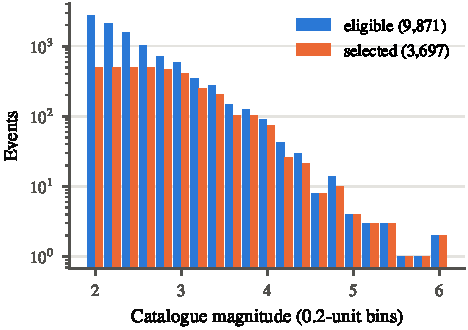
\includegraphics[width=0.6\textwidth]{figures/fig_selection.pdf}
\caption{Magnitude distribution of events with at least three accepted
records (eligible) and of the balanced selection (logarithmic scale).}
\label{fig:selection}
\end{figure}

\subsection{Predictive skill}
Table~\ref{tab:skill} compares the feature sets. Source--station geometry alone
reduces the error relative to the constant predictor, reflecting that larger
events are recorded at larger distances. The amplitude-independent
descriptors reduce the event-level MAE from 0.392 to 0.343, which is
32\,\% of the difference between the geometry-only and amplitude reference
models. Removing the controls changes the shape model only marginally.
Figure~\ref{fig:pred} shows the event-level predictions.

\begin{table}[ht]
\centering\small
\caption{Event-level skill (mean $\pm$ s.d.\ over 15 doubly disjoint folds,
$\approx 564$ test events per fold). Record-level MAE in the last column.}
\label{tab:skill}
\begin{tabular}{lccccc}
\toprule
Feature set & MAE & RMSE & $R^2$ & Spearman $\rho$ & MAE (records) \\
\midrule
Constant (training mean) & 0.466 & -- & -- & -- & -- \\
Controls only & $0.392\pm0.016$ & 0.525 & 0.21 & 0.49 & 0.446 \\
Shape only & $0.347\pm0.018$ & 0.452 & 0.42 & 0.63 & 0.369 \\
\textbf{Shape + controls} & $\mathbf{0.343\pm0.017}$ & \textbf{0.446} & \textbf{0.43} & \textbf{0.64} & \textbf{0.365} \\
Amplitude reference & $0.238\pm0.022$ & 0.305 & 0.73 & 0.84 & 0.279 \\
\bottomrule
\end{tabular}
\end{table}

\begin{figure}[ht]
\centering
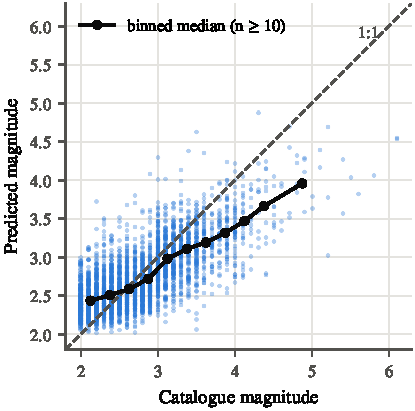
\includegraphics[width=0.5\textwidth]{figures/fig_pred_vs_true.pdf}
\caption{Predicted versus catalogue magnitude for the shape model (event
median over stations, averaged over repeats; 3\,561 events).}
\label{fig:pred}
\end{figure}

\subsection{Magnitude-dependent bias}
All models regress towards the mean of the training distribution
(Table~\ref{tab:bias}, Figure~\ref{fig:bias}). Events at $M\,2.0$--$2.5$ are
overestimated by 0.2--0.4 units, partly because no smaller events exist in the
catalogue to balance them. Above $M\,3.5$ the shape model underestimates
increasingly, by $-0.67$ at $M\,4.0$--$4.5$ and $-1.01$ above $M\,4.5$. This
is less than the geometry-only model but more than the amplitude reference.
Near the centre of the distribution ($M\,2.5$--$3.0$) the geometry-only model
attains a lower MAE than the shape model, which is consistent with its
predictions concentrating near the mean.

\begin{table}[ht]
\centering\small
\caption{Event-level bias (predicted $-$ catalogue) and MAE by magnitude bin.}
\label{tab:bias}
\begin{tabular}{lrrrrrrr}
\toprule
& & \multicolumn{2}{c}{Shape + controls} & \multicolumn{2}{c}{Controls only} & \multicolumn{2}{c}{Amplitude ref.} \\
\cmidrule(lr){3-4}\cmidrule(lr){5-6}\cmidrule(lr){7-8}
Bin & $n$ & bias & MAE & bias & MAE & bias & MAE \\
\midrule
2.0--2.5 & 1186 & $+0.29$ & 0.31 & $+0.38$ & 0.38 & $+0.20$ & 0.22 \\
2.5--3.0 & 1161 & $-0.07$ & 0.22 & $-0.09$ & 0.15 & $-0.03$ & 0.17 \\
3.0--3.5 & 757 & $-0.16$ & 0.28 & $-0.30$ & 0.34 & $-0.08$ & 0.19 \\
3.5--4.0 & 306 & $-0.44$ & 0.48 & $-0.73$ & 0.73 & $-0.26$ & 0.29 \\
4.0--4.5 & 109 & $-0.67$ & 0.69 & $-1.17$ & 1.17 & $-0.39$ & 0.40 \\
$\geq 4.5$ & 42 & $-1.01$ & 1.01 & $-1.89$ & 1.89 & $-0.42$ & 0.45 \\
\bottomrule
\end{tabular}
\end{table}

\begin{figure}[ht]
\centering
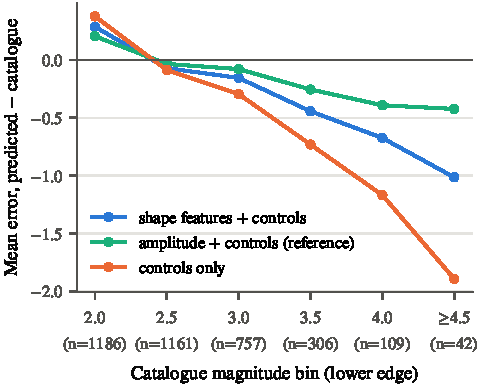
\includegraphics[width=0.55\textwidth]{figures/fig_bias.pdf}
\caption{Mean event-level error by magnitude bin for the three models.}
\label{fig:bias}
\end{figure}

\subsection{Descriptor importance}
In the Shapley analysis, the event-median attenuation-corrected corner
frequency of the P wave had the largest mean absolute contribution (0.18
magnitude units), followed by epicentral distance (0.12) and the
corresponding S-wave corner frequency (0.12). Permutation of single
quantities (Figure~\ref{fig:importance}b) ranks epicentral distance first
($\Delta$MAE $0.039\pm0.009$) and the P corner frequency second ($0.020\pm0.008$,
positive in all 15 folds), followed by the misfit of the attenuation-corrected
S-wave source fit, the S corner frequency, and the LPDT plateau time.

Single-quantity permutation understates correlated quantities that can
substitute for each other. Shuffled jointly (Figure~\ref{fig:importance}a), the
P and S corner frequencies increase the MAE by $0.086\pm0.012$, exceeding all
distance controls together ($0.073\pm0.015$); adding the remaining corner
estimates and P/S ratios does not increase this value (0.084). The LPDT
measures together contribute $0.008\pm0.004$. All four concept effects were
positive in every fold. Because permutation substitutes misleading values
rather than removing a feature, these increases measure the model's reliance on
a descriptor, not the loss expected after retraining without it.

The source-fit misfit has almost no correlation with magnitude by itself
(partial Spearman $\rho = 0.01$ at fixed distance). Its importance therefore
probably reflects an interaction: the misfit informs the model about the
reliability of the corner-frequency estimate on a given record.

\begin{figure}[ht]
\centering
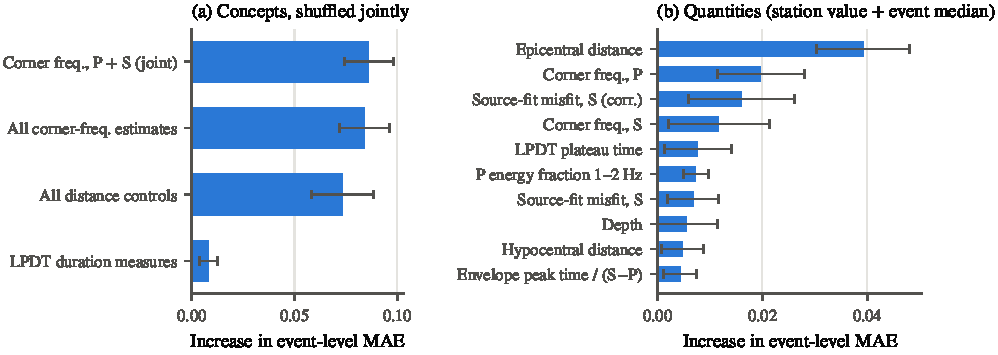
\includegraphics[width=\textwidth]{figures/fig_importance.pdf}
\caption{Grouped permutation importance (increase in event-level MAE; mean
$\pm$ s.d.\ over 15 folds). (a) Substitutable quantities shuffled jointly.
(b) Ten most important quantities, each shuffled together with its event median.}
\label{fig:importance}
\end{figure}

\subsection{Corner-frequency scaling}
The event-median apparent corner frequency decreases with magnitude for both
phases (Figure~\ref{fig:fc}; Spearman $\rho = -0.55$ for P and $-0.49$ for S).
The fitted slopes of $\log_{10}\fc$ against magnitude are $-0.13$ (P) and
$-0.11$ (S), and the medians lie between about 2 and 5\,Hz. Self-similar
scaling implies $-0.5$ per unit $M_w$; even allowing for the faster growth of
$M_L$ relative to $M_w$ at small magnitudes \citep{deichmann2006}, the observed
slope is several times shallower. Moreover, corner frequencies of a few hertz
are low for $M\,2$--$3$ earthquakes. The estimate is therefore an apparent,
band-limited quantity that retains the ordering of source size but compresses
its range.

\begin{figure}[ht]
\centering
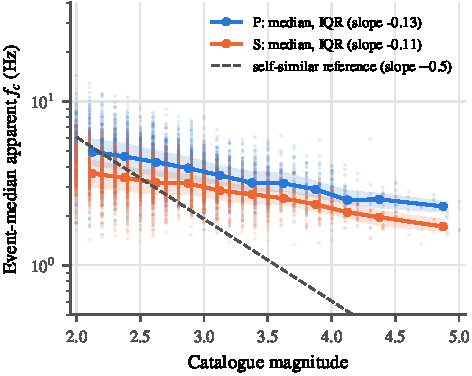
\includegraphics[width=0.55\textwidth]{figures/fig_fc_scaling.pdf}
\caption{Event-median apparent corner frequency (Eq.~\ref{eq:snoke}) against
magnitude; points are events, lines and bands are bin medians and
interquartile ranges. The dashed line shows the self-similar slope for
comparison, anchored arbitrarily at $M\,2.5$.}
\label{fig:fc}
\end{figure}

\subsection{Sensitivity experiments}
Two variants were evaluated on the same folds (Table~\ref{tab:sens}).
\emph{Tail weighting}, which multiplies record weights by the inverse
frequency of the magnitude bin (capped at 10), reduced the underestimation of large
events only modestly ($-0.57$ instead of $-0.67$ at $M\,4.0$--$4.5$) while
increasing the overall MAE. Thus, sample imbalance alone does not explain the
bias. \emph{Restricting training and testing to $M_L$ events}
removed 246 $M_w$ events (median $M\,4.0$). On the same $M_L$ events its MAE
($0.302\pm0.016$) did not differ meaningfully from the default model
($0.314\pm0.015$), while its underestimation above $M\,3$ increased because
fewer large events remained for training. Mixing the two scales is therefore not
the main limitation.

\begin{table}[ht]
\centering\small
\caption{Sensitivity experiments (shape + controls; event-level MAE).}
\label{tab:sens}
\begin{tabular}{lccc}
\toprule
Variant & All test events & Subset & Bias $M\,4.0$--$4.5$ \\
\midrule
Default & $0.343\pm0.017$ & $M_w$ events: $0.687\pm0.061$ & $-0.67$ \\
Tail weighting & $0.367\pm0.019$ & $M_w$ events: $0.609\pm0.054$ & $-0.57$ \\
\midrule
Default, $M_L$ events only & -- & $0.314\pm0.015$ & -- \\
$M_L$-only model & $0.302\pm0.016$ & -- & -- \\
\bottomrule
\end{tabular}
\end{table}

\section{Discussion and limitations}

The results indicate that waveform descriptors which are invariant to
amplitude and insensitive to station SNR still carry substantial information
on earthquake size, and that this information is concentrated in a single
physical quantity, the attenuation-corrected corner frequency aggregated over
the network. That a data-driven ranking recovers the quantity predicted by
source theory supports the interpretation that the model learns source
properties rather than shortcuts. The audit was essential to this
interpretation: several descriptors with high apparent relevance, in
particular high-frequency spectral and complexity measures, followed station
SNR within events and were excluded.

The main limitation is the compressed magnitude scaling of the apparent
corner frequency and the resulting underestimation of larger events. Three
causes are plausible and not yet separated: (i) window length: the 2\,s P and
5\,s S windows limit the spectral resolution (0.5 and 0.2\,Hz) and the
observable source duration, which affects the larger events most; (ii) the
fixed regional $Q(f)$ and the uncorrected site $\kappa$, which bias the
corner frequency towards lower values for small events; and (iii) the
analysis band (0.7 or 1 to 40\,Hz), which truncates corners above
the anti-alias range. Further limitations are the mixture of $M_L$ and $M_w$
labels; the whole-second origin times; the catalogue lower limit at $M\,2.0$,
which produces the bias at the low end; the residual, sub-threshold SNR
sensitivity of the retained descriptors; and the choice of the threshold
$\lambda = 0.15$, $Q(f)$ and the window lengths, whose influence on the
conclusions has not yet been tested. The study covers approximately 16 months
of data from one network, and the dominant role of distance is partly a
consequence of recording selection.

\section{Conclusions and future work}

Under a design that excludes amplitude, its proxies, shared events and shared
stations, gradient-boosted trees recover about one third of the gap between a
geometry-only model and an amplitude-based reference. The network-median,
attenuation-corrected corner frequency of P and S waves is the dominant
amplitude-independent descriptor of earthquake size, although its observed
scaling is far shallower than self-similar theory predicts. Planned work:
(1) multiple and longer analysis windows to test whether the saturation at
larger magnitudes is a resolution effect; (2) sensitivity analyses of $Q(f)$,
site $\kappa$, the leakage threshold and window lengths, and region- and
sequence-held-out validation; (3) extension to a second network and period;
(4) an early-warning variant restricted to the first seconds of P; and (5) a
systematic literature review with full-text access.

\section*{Data and code availability}
The processing and analysis code, including automated tests and complete
feature definitions, is maintained in the project repository. Waveforms are
available from the KOERI network \citepalias{koeri_ko} and hypocentres from AFAD
\citepalias{afad_catalog}.

\section{Declaration of AI use}
\label{sec:ai}

Generative AI was used extensively in this work. The AI system was Claude Opus 5.5 (Anthropic),
accessed through the Claude Code command-line agent, in October 2026. It was used for:
\begin{enumerate}
\item \textbf{Software}: design and implementation of the data-processing,
  feature-extraction, event-selection, training and evaluation code and its
  automated tests, at the author's direction;
\item \textbf{Analysis}: execution of the experiments, the leakage audit and
  the importance analyses, and production of all figures and tables;
\item \textbf{Literature}: identification of candidate references by web
  search and verification of their bibliographic data against Crossref and
  publisher records. Because institutional access was unavailable, the full
  texts were \emph{not} read by the author or by the AI system; statements
  about cited works rest on abstracts, metadata and general domain knowledge,
  and two bibliographic errors in the AI's own recollection were found and
  corrected during verification;
\item \textbf{Writing}: drafting of this manuscript.
\end{enumerate}
The research question and the main methodological decisions were set by the
author. These decisions include requiring amplitude independence, adding
physics-based descriptors, excluding SNR-sensitive descriptors by default,
balancing magnitudes and reporting only leakage-filtered results.
All numerical results were produced by the code in the project
repository and can be regenerated from it. The author has reviewed this
AI-drafted preliminary report and takes responsibility for its content.
Before any formal use, the literature claims will be checked against the
original publications and the manuscript revised in the author's own words.

\bibliographystyle{plainnat}
\bibliography{refs}

\appendix
\section{Retained descriptors}
\label{app:features}
\small
\begin{tabularx}{\textwidth}{lL}
\toprule
Family & Descriptors (prefix \code{f_} omitted) \\
\midrule
P spectrum & \code{pz_centroid_hz}, \code{pz_frac_1_2}, \code{pz_frac_2_4}, \code{pz_frac_4_8}, \code{pz_frac_8_16}, \code{pz_peak_hz}, \code{pz_rolloff50_hz} \\
S spectrum & \code{sh_centroid_hz}, \code{sh_entropy}, \code{sh_frac_1_2}, \code{sh_frac_2_4}, \code{sh_frac_4_8}, \code{sh_frac_8_16}, \code{sh_peak_hz}, \code{sh_rolloff50_hz}, \code{sh_rolloff85_hz}, \code{sh_rolloff95_hz} \\
P source & \code{pz_snoke_fc_hz}, \code{pz_boat_rms}, \code{pz_fc_at_edge} \\
P source (att.-corr.) & \code{pz_qc_snoke_fc_hz}, \code{pz_qc_boat_rms}, \code{pz_qc_fc_at_edge} \\
S source & \code{sh_snoke_fc_hz}, \code{sh_boat_rms}, \code{sh_brune_rms}, \code{sh_fc_at_edge} \\
S source (att.-corr.) & \code{sh_qc_snoke_fc_hz}, \code{sh_qc_boat_rms}, \code{sh_qc_brune_rms}, \code{sh_qc_fc_at_edge} \\
Corner ratios & \code{fc_p_over_s_brune}, \code{fc_p_over_s_snoke} \\
LPDT & \code{lpdt_t_plateau_s}, \code{lpdt_slope_dec_per_s}, \code{lpdt_t90_s} \\
Peak-ratio periods & \code{pz_T_va_s}, \code{sh_T_va_s} \\
Statistics & \code{pz_abs_skew}, \code{pz_crest}, \code{sh_abs_skew}, \code{sh_crest} \\
Polarisation & \code{ppol_incidence_deg}, \code{ppol_log_h_over_v}, \code{spol_incidence_deg}, \code{spol_log_h_over_v}, \code{spol_planarity}, \code{spol_rectilin} \\
Envelope (horizontal) & \code{envh_decay_powerlaw}, \code{envh_rise_10_90_s}, \code{envh_t_peak_rel_sp}, \code{envh_t_peak_s} \\
\midrule
Event medians & \code{pz_qc_snoke_fc_hz}, \code{sh_qc_snoke_fc_hz}, \code{lpdt_t_plateau_s}, \code{fc_p_over_s_snoke} \\
Controls & epicentral and hypocentral distance, depth, back-azimuth, theoretical S--P time \\
\bottomrule
\end{tabularx}

\end{document}
